\documentclass[a4paper,12pt]{article}
\usepackage[utf8]{inputenc}
\usepackage[spanish]{babel}
\usepackage{color}
\usepackage{parskip}
\usepackage{graphicx}
\usepackage{multirow}
\usepackage{listings}
\usepackage{vmargin}
\usepackage{datetime}
\newdate{date}{19}{10}{2017}
\graphicspath{ {imagenes/} }
\definecolor{mygreen}{rgb}{0,0.6,0}
\definecolor{lbcolor}{rgb}{0.9,0.9,0.9}
\usepackage{epstopdf}
\usepackage{float}


\setpapersize{A4}
\setmargins{2.5cm}       % margen izquierdo
{1.5cm}                        % margen superior
{16.5cm}                      % anchura del texto
{23.42cm}                    % altura del texto
{10pt}                           % altura de los encabezados
{1cm}                           % espacio entre el texto y los encabezados
{0pt}                             % altura del pie de página
{2cm}     

\lstset{
    tabsize=4,    
%   rulecolor=,
    language=[GNU]C++,
        basicstyle=\tiny,
        aboveskip={1.5\baselineskip},
        columns=fixed,
        showstringspaces=false,
        extendedchars=false,
        breaklines=true,
        prebreak = \raisebox{0ex}[0ex][0ex]{\ensuremath{\hookleftarrow}},
        frame=single,
        showtabs=false,
        showspaces=false,
        showstringspaces=false,
        identifierstyle=\ttfamily,
        keywordstyle=\color[rgb]{0,0,1},
        commentstyle=\color[rgb]{0.026,0.112,0.095},
        stringstyle=\color{red},
        numberstyle=\color[rgb]{0.205, 0.142, 0.73},
%        \lstdefinestyle{C++}{language=C++,style=numbers}’.
}


\begin{document}
\title{Algoritmo para hacer Líneas}
\author{
Christofer Fabián Chávez Carazas \\
\small{Universidad Nacional de San Agustín de Arequipa} \\
\small{Escuela Profesional de Ciencia de la Computación} \\
\small{Computación Gráfica}
}
\date{\displaydate{date}}

\maketitle

\begin{large}
 \textbf{Problema}
\end{large}

\textbf{Programar un algoritmo propio para dibujar líneas}

En el principio del algoritmo se verifica si la línea es recta. Si no lo es se pasa a la siguiente parte.
Ahí se verifica a qué dirección va a ir la recta y en base a qué eje se van a pintar los tramos.
Cada tramo tiene un tamaño del eje más largo entre el eje mas corto. Cada vez que se pinta un tramo
se acumula en una variable los decimales de la anterior división. Si esta variable es mayor de uno, entonces
el tramo en el que se encuentra aumenta su tamaño en uno.


\begin{lstlisting}
#include <GL/glut.h>
#include <iostream>
#include <cmath>
#include <algorithm>
#include <tuple>

using namespace std;

enum Direcciones {ARRIBA,ABAJO,DERECHA,IZQUIERDA};


void init(void){
    glClearColor(1.0,1.0,1.0,0.0);
    glMatrixMode(GL_PROJECTION);
    gluOrtho2D(0.0,400.0,0.0,300.0);
}

void drawPoint(int x, int y){
    glBegin(GL_POINTS);
        glVertex2i(x,y);
    glEnd();
}

tuple<int,int> getDir(int x1, int y1, int x2, int y2){
    int dirX = -1;
    int dirY = -1;
    if(x1 < x2) dirX = DERECHA;
    else dirX = IZQUIERDA;
    if(y1 < y2) dirY = ARRIBA;
    else dirY = ABAJO;
    return make_tuple(dirX,dirY);
}

void drawLine(int x1, int y1, int x2, int y2){
    if(x1 == x2){
        int yMin = min(y1,y2);
        int yMax = max(y1,y2);

        for(int i = yMin; i <= yMax; i++){
            drawPoint(x1,i);
        }
    }
    else if(y1 == y2){
        int xMin = min(x1,x2);
        int xMax = max(x1,x2);
        for(int i = xMin; i <= xMax; i++){
            drawPoint(i,y1);
        }
    }
    else{
        int dirX = -1;
        int dirY = -1;
        tie(dirX,dirY) = getDir(x1,y1,x2,y2);
        int ejeMax = max(abs(x1-x2) + 1,abs(y1-y2) + 1);
        int ejeMin = min(abs(x1-x2) + 1,abs(y1-y2) + 1);
        float saltosF = (float)ejeMax / (float)ejeMin;
        int saltos = saltosF;
        float decimalesSaltos = saltosF - saltos;
        float decimalActual = 0;
        int direcX = 1;
        int direcY = 1;
        int actualX = x1;
        int actualY = y1;
        if(dirX == IZQUIERDA) direcX = -1;
        if(dirY == ABAJO) direcY = -1;
        if(ejeMax == abs(x1-x2) + 1){
            for(actualY = y1; actualY != y2 + direcY; actualY = actualY + direcY){
                for(int i = 0; i < saltos; i++){
                    drawPoint(actualX,actualY);
                    if(actualX == x2) break;
                    actualX = actualX + direcX;
                }
                decimalActual+= decimalesSaltos;
                if(actualX == x2) break;
                if(decimalActual >= 1){
                    drawPoint(actualX,actualY);
                    if(actualX == x2) break;
                    actualX = actualX + direcX;
                    decimalActual -= 1;
                }
            }
            actualY = y2;
            while(actualX != x2){
                actualX = actualX + direcX;
                drawPoint(actualX,actualY);
            }
        }
        else{
            for(actualX = x1; actualX != x2 + direcX; actualX = actualX + direcX){
                for(int i = 0; i < saltos; i++){
                    drawPoint(actualX,actualY);
                    if(actualY == y2) break;
                    actualY = actualY + direcY;
                }
                decimalActual+= decimalesSaltos;
                if(actualY == y2) break;
                if(decimalActual >= 1) {
                    drawPoint(actualX,actualY);
                    if(actualY == y2) break;
                    actualY = actualY + direcY;
                    decimalActual -= 1;
                }

            }
            actualX = x2;
            while(actualY != y2){
                actualY = actualY + direcY;
                drawPoint(actualX,actualY);
            }   
        }
    }
}

void display(){
    glClear(GL_COLOR_BUFFER_BIT);
    glColor3f(1.0,0.0,0.0);
    drawLine(20,20,200,25);
    glColor3f(0.0,0.0,0.0);
    glBegin(GL_LINES);
        glVertex2i(20,20);
        glVertex2i(200,25);
    glEnd();
    glFlush();
}

int main(int argc, char **argv)
{
    glutInit(&argc,argv);
    glutInitDisplayMode(GLUT_SINGLE | GLUT_RGB);
    glutInitWindowPosition(50,100);
    glutInitWindowSize(400,300);
    glutCreateWindow("Ejemplo");
    init();
    glutDisplayFunc(display);
    glutMainLoop();
    
}
\end{lstlisting}

\begin{large}
 \textbf{Resultados}
\end{large}

\begin{figure}[H]
 \centering
 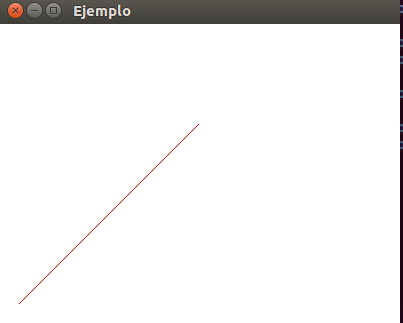
\includegraphics[scale = 0.5]{1.png}
\end{figure}
\begin{figure}[H]
 \centering
 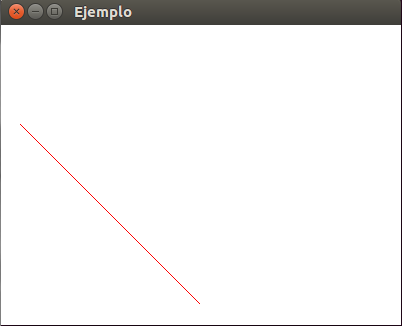
\includegraphics[scale = 0.5]{2.png}
\end{figure}
\begin{figure}[H]
 \centering
 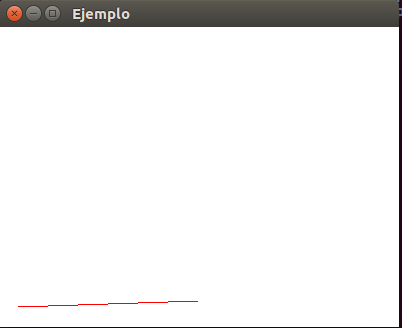
\includegraphics[scale = 0.5]{3.png}
\end{figure}
\begin{figure}[H]
 \centering
 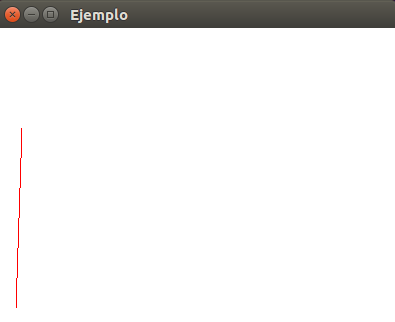
\includegraphics[scale = 0.5]{4.png}
\end{figure}




\end{document}

